\subsection{Results and discussion}\label{sec:m3:results}
    We present the results of the numerical solutions of the Einstein-Boltzmann equations and discuss them in due order starting with the potentials, then the multipoles and finally the matter perturbations. The main focus is on the evolution of these perturbations, leaving the discussion of the initial conditions for the next section. 

\subsubsection{Potentials}
    ~\cref{fig:m3:potentials} shows the metric perturbation potentials $\Phi$ and $\Psi$ as functions of time $x$ for the $k$-modes under investigation. The time of matter-radiation equality and recombination is marked in the plot as black dash-dotted and a shaded grey area respectively. Let's first consider the top panel, showing only $\Phi$. At early times, it is constant across all $k$-modes. \footnote{When referring to ``all $k$-modes'' it is implicit that we only mean the three modes considered here, but the qualitative discussions should be valid across all $k$-modes.} This is expected since at early times, the horizon is small and most modes are larger than this. Thus, they will be unaffected by causal physics and stay constant at their initial value. As time proceeds, the smaller $k$-modes will enter the horizon and are suddenly subjected to causal physics. We see from the top panel that if this happens in the radiation dominated regime (before radiation-matter equality), the potential will decline as $e^{-2x}$. This can be seen from ~\cref{eq:m3:theory:phi_perturbation}. In addition, the damped oscillations predicted by ~\cref{eq:m3:theory:analytical_small_scales_radiation_domination} are clearly seen for these scales. The smaller the scale, the earlier it crosses the horizon, and the more suppression, oscillation and damping it experiences. In order to explain the physics behind this we must consider the primordial baryon-photon plasma which exert a radiation pressure, which is the dominant component of the universe at this time (hence radiation domination). This pressure counteracts gravitational forces and will prevent overdensities of the photon-baryon fluid from growing, effectively making the potential decay as a result of an expanding universe. The main source of the potential in the radiation era is thus the dark energy, of which we have a constant amount that does not couple to photons nor baryons. Therefore, if the universe expands as $\sim a^2=e^{2x}$,\footnote{Valid in the radiation dominated era since $a(t) \propto t^{1/2}$ in this regime.} the potential must decay as the inverse. As this decay happen, the potential will experience oscillations due to the interplay between accretion of baryons in gravitational wells, and the counter-acting radiation pressure.  
    
    However, for large scale modes, like the blue graph, where horizon crossing happens in the matter dominated regimes, then we expect the potential to change with a factor $9/10$ as it transitions from radiation domination to matter domination, from ~\cref{eq:m3:theory:analytical_large_scale_super_horizon}. If modes cross the horizon during matter domination then the potential stays constant. This is because the expansion factor of the universe during matter domination balances the accretion of matter in overdense regions. This is further emphasised after recombination when baryons decouple from photons and evolve with dark matter instead, not being subjected to the radiation pressure. 
    
    The sum of the potentials in the bottom panel of ~\cref{fig:m3:potentials} goes as $\Psi+\Phi \sim e^{-2x}/k^2\T_2$, so it will closely follow the quadrupole term, but being suppressed by an exponential factor. Also, the $k^2$ term suggested larger value for small $k$-s (large scale). We save the discussion of the quadrupole, but the latter can clearly be seen as the large and intermediate scale modes show sinusoidal behaviour, with the large scale mode having a larger amplitude. Both are exponentially suppressed. These effects happen when the tight coupling epoch is over, since all multipoles except the monopole and dipole are suppressed during tight coupling. 
    \begin{figure}
        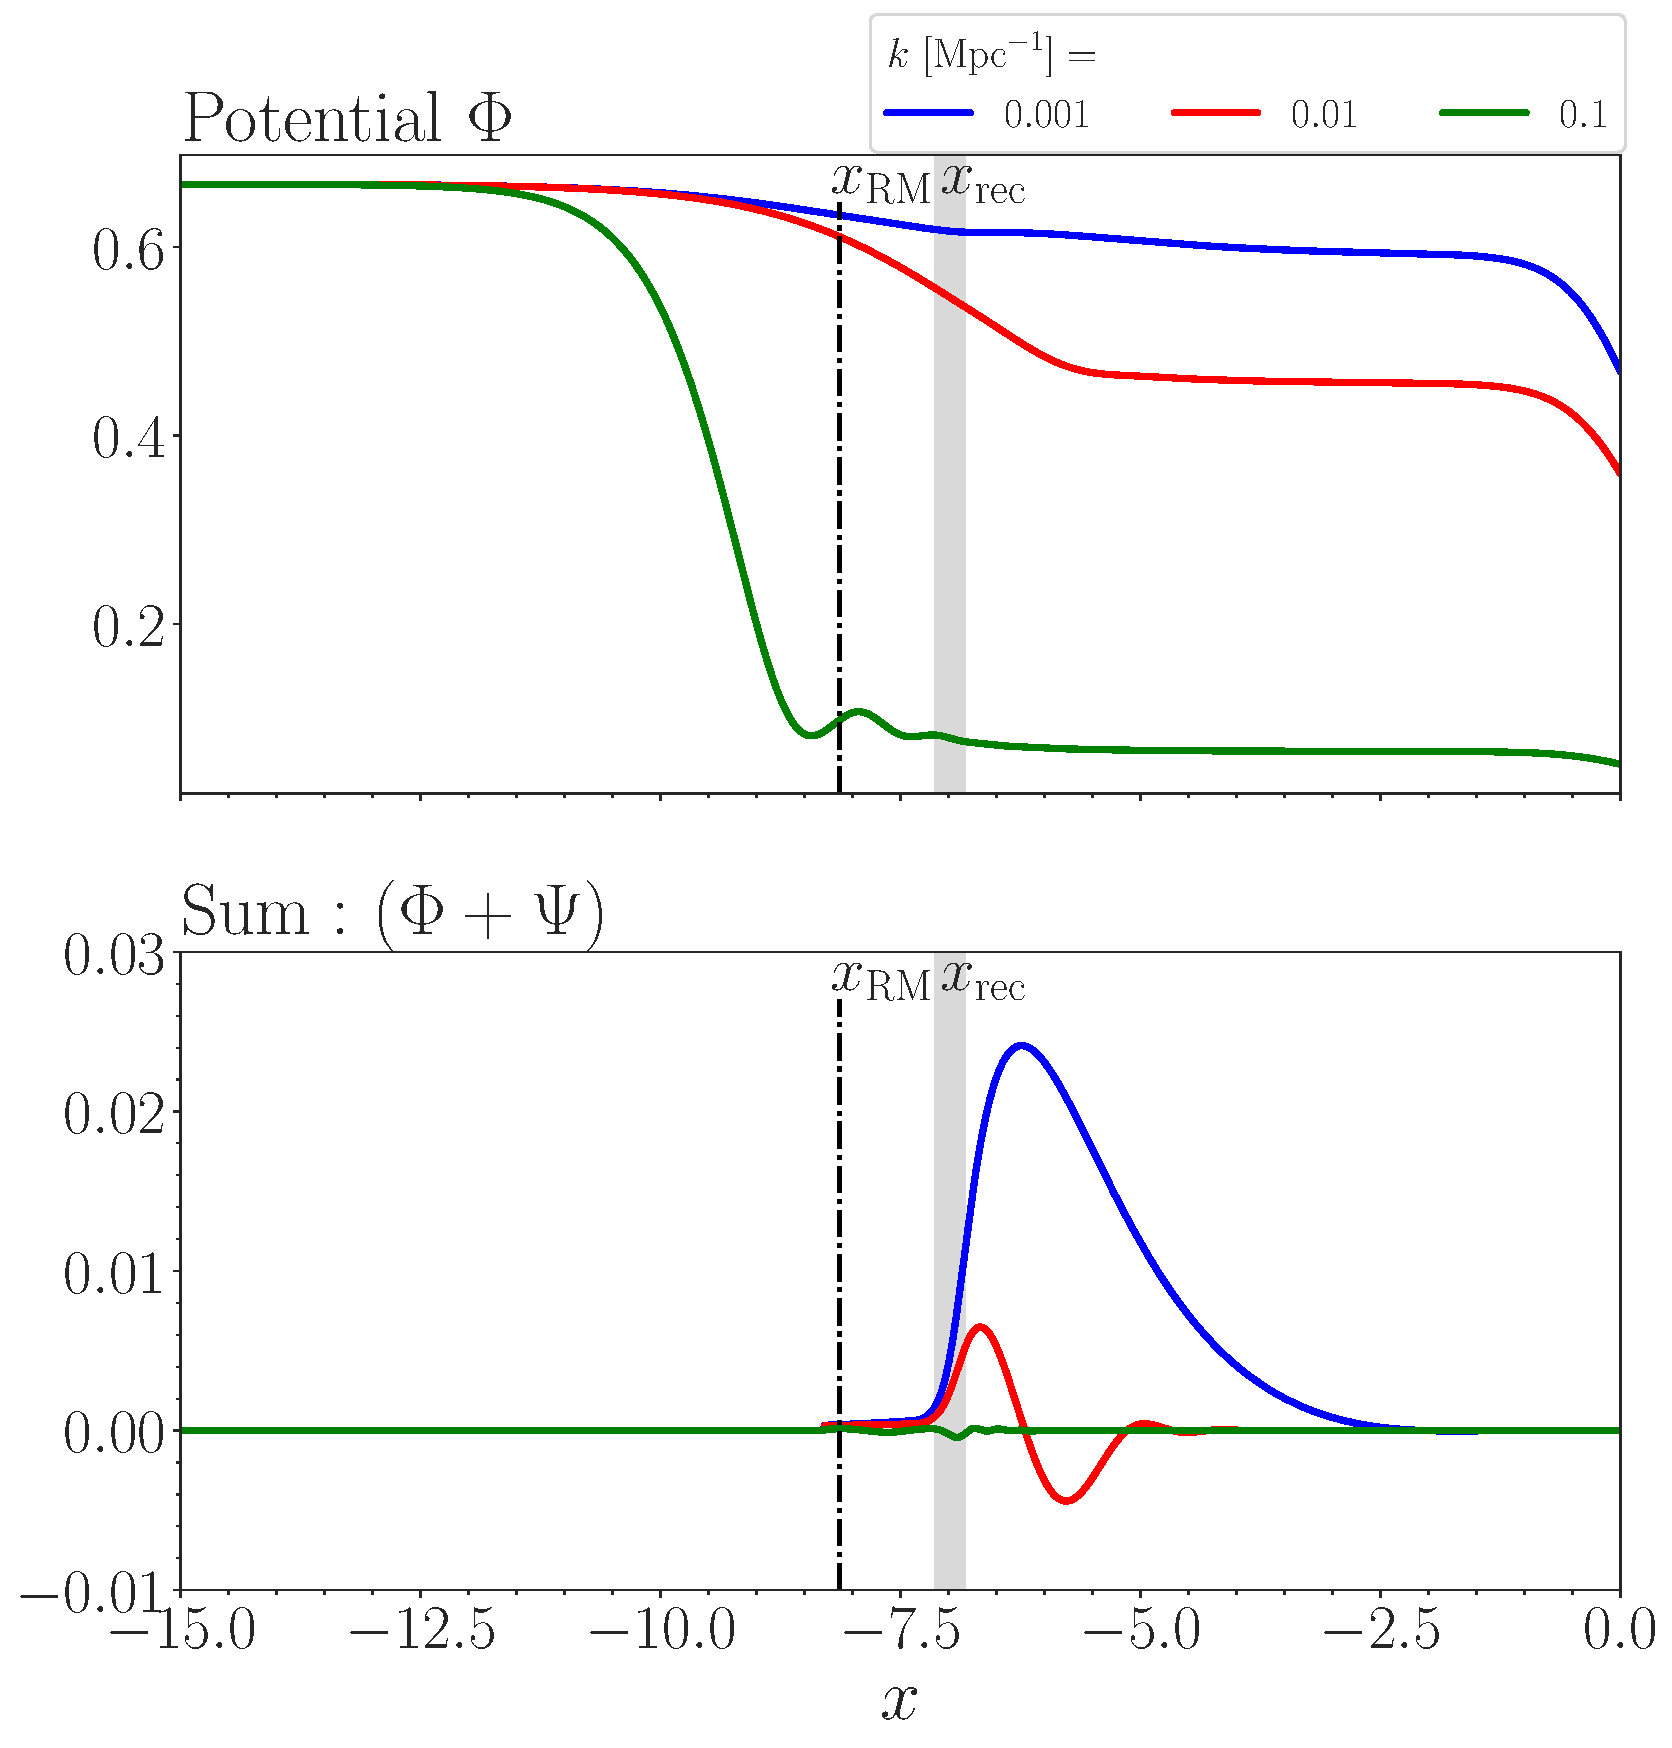
\includegraphics[width=\linewidth]{potentials.pdf}
        \caption{The metric perturbation potentials, $\Psi$ representing the Newtonian potential, and $\Phi$ representing the spatial curvature perturbation. Both panels show the evolution as function of the time $x$, for the three different $k$-modes outlined in ~\cref{sec:m3:methods}. The top panel shows $\Phi$ alone, while the bottom shows the sum of the two. The grey shaded are represent the time of recombinaiton as found in ~\cref{sec:m2}, highlighting the fact that it did not occur in an instant, and the dash-dotted black line is the time of radiation-matter equality as found in ~\cref{sec:m1}.}
        \label{fig:m3:potentials}
    \end{figure}

\subsubsection{Multipoles}
    We now focus our attention on the multipoles, starting with the monopole term expressed through the photon overdensity $\delta_\gamma = 4\T_0$. Mathematically, this relation can be seen  from either the parenthesis in ~\cref{eq:m3:theory:time_evolution_of_Phi} or the definition of $\mathcal{Y}$ in ~\cref{eq:m3:theory:metric_perturbations_final} following somewhat diffuse symmetry arguments. Physically it also makes sense since the photon monopole is some measure of the average photon temperature which intuitively can be though of as a photon overdensity. It can be seen for the various $k$-modes in ~\cref{fig:m3:monopole}, where we clearly see that the small scale perturbation undergoes horizon crossing first, and become subject to causal physics. This is manifest in the oscillation of the green curve in the figure. Metric perturbations and pressure will generate acoustic oscillations within causally connected regions. When the horizon increase, these oscillations will affect a spatially large area, affecting $k$-modes on larger and larger scales. This is also manifest in ~\cref{fig:m3:monopole} as the intermediate $k$-mode starts to oscillate later, and finally the large scale mode. 

    What are the monopole fluctuations really? The different modes represent the average temperature at different physical length scales. At early times, when the horizon is small, most modes are outside it, leaving their average temperature and thus monopole constant. As modes enter the horizon, they become subject to causal physics, like the gravitational potential. Since photons and baryons are coupled at early times, photons must continuously climb in and out of the gravitational potential wells set up by matter, gaining and loosing energy in the process. It is worth noticing that this manifest itself as oscillations in Fourier space, but can be interpreted as propagating acoustic waves in real space. Before recombination, for modes having entered the horizon, these are waves in the baryon-photon fluid, propagating with the speed of sound. The origin of these oscillations in the radiation era is the decay of the gravitational potentials (discussed in the previous section), an effect called \textit{radiation driving}. The oscillations are also asymmetric about its equilibrium position. This is due to \textit{baryon loading} where the potentials change slightly because of the oscillating baryons, whereas the radiation pressure is left unchanged. The fact that the baryons and photons move together affects the sound speed which also causes some asymmetry to the oscillations. After recombination, photons decouple from baryons and stream freely throughout the Universe. During this decoupling process the interaction rate between photons and baryons decreases, but does not become zero. There as still interactions, causing energy to be transported and, temperature fluctuations on small scales to become washed out. This is known as diffusion damping, and smooths out the small scale perturbation for both radiation and matter. This is manifest for the small scale mode in green in ~\cref{fig:m3:monopole} as its amplitude decays after recombination. This phenomenon is not present for the modes entering the horizon after decoupling, in the matter regime. 

    Thus, the photon monopole perturbation behaves somewhat according to ~\cref{eq:m3:theory:analytical_monopole_eom}, where the oscillations are sourced by some force term which is a function of the potentials. This is true before decoupling for modes having entered the horizon. Super-horizon modes hardly evolve at all, due to the lack of causal physics.
    \begin{figure}
        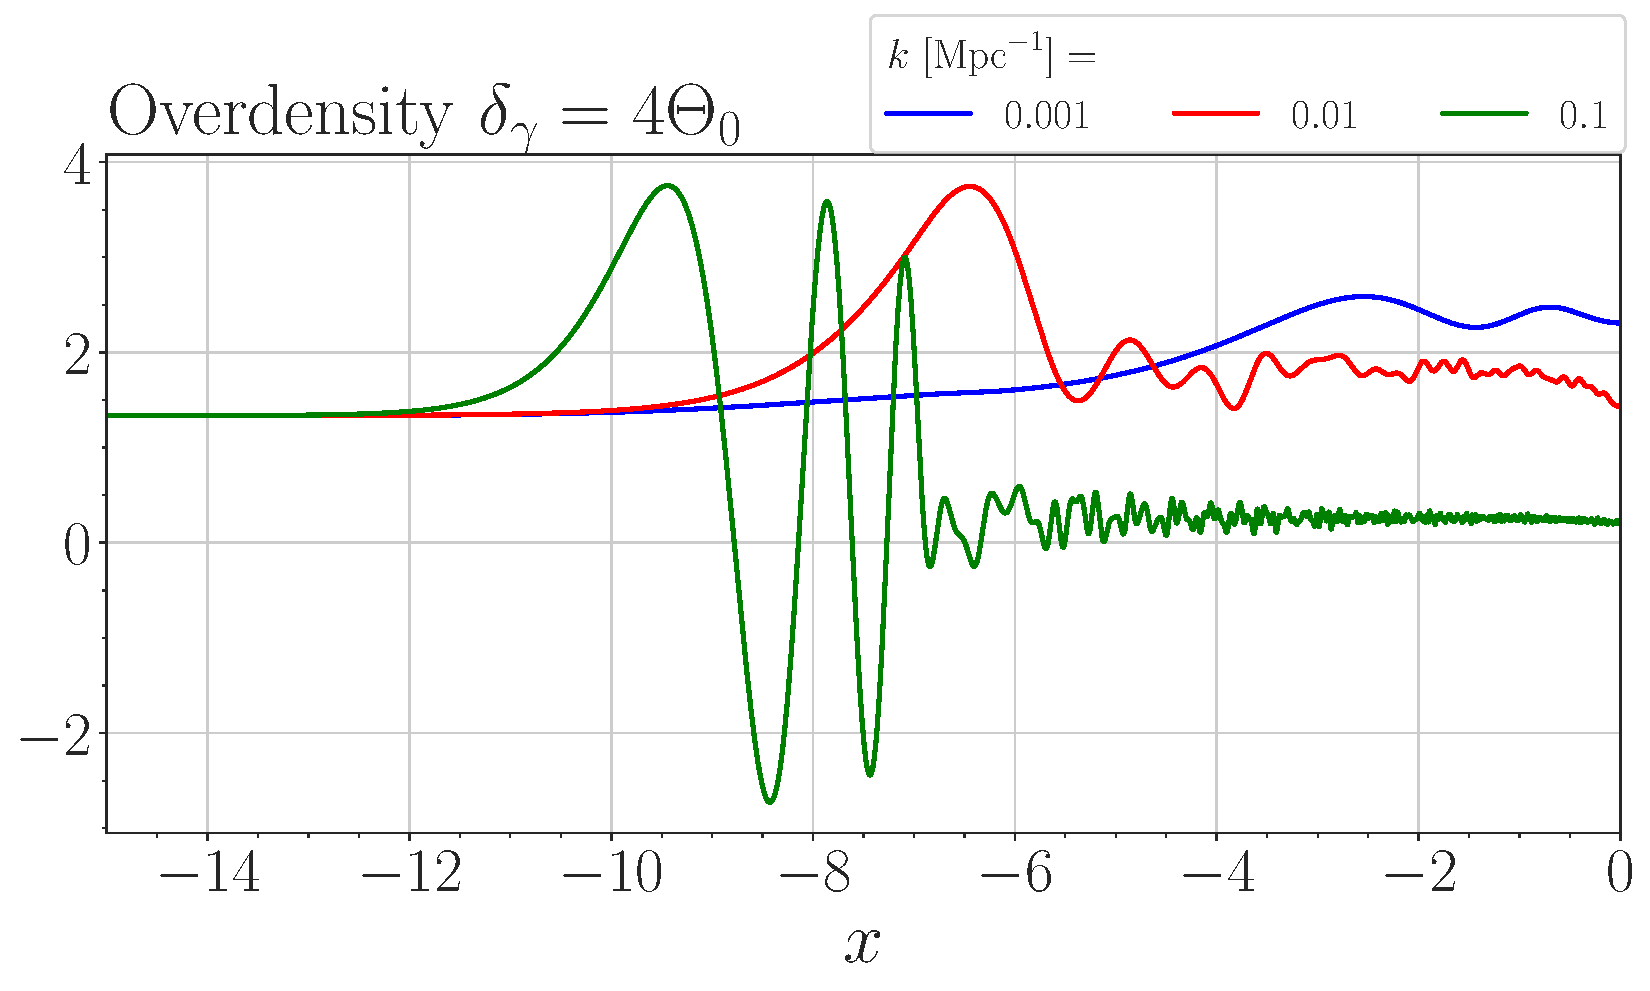
\includegraphics[width=\linewidth]{monopole.pdf}
        \caption{Photon overdensity represented by the photon monopole for the various $k$-modes. Recombination is marked as a shaded grey area. The time of radiation-matter equality is marked with a dashed black line.}
        \label{fig:m3:monopole}
    \end{figure}

    A similar discussion to the one above can be applied on the photon velocity $v_\gamma = -3\T_1$, as shown in ~\cref{fig:m3:dipole}. Similarly to the monopole, small scale modes enter the horizon first and starts to oscillate followed by larger scale modes. Modes entering the horizon before recombination experience diffusion damping, effectively smoothing the average velocity of the photons. Worth noticing in this plot is that for similar modes, the oscillatory behaviour of the photon velocity is starting slightly before the overdensity. This makes sense, since we need something to be moving in the first place for overdensities to occur. 

    \begin{figure}
        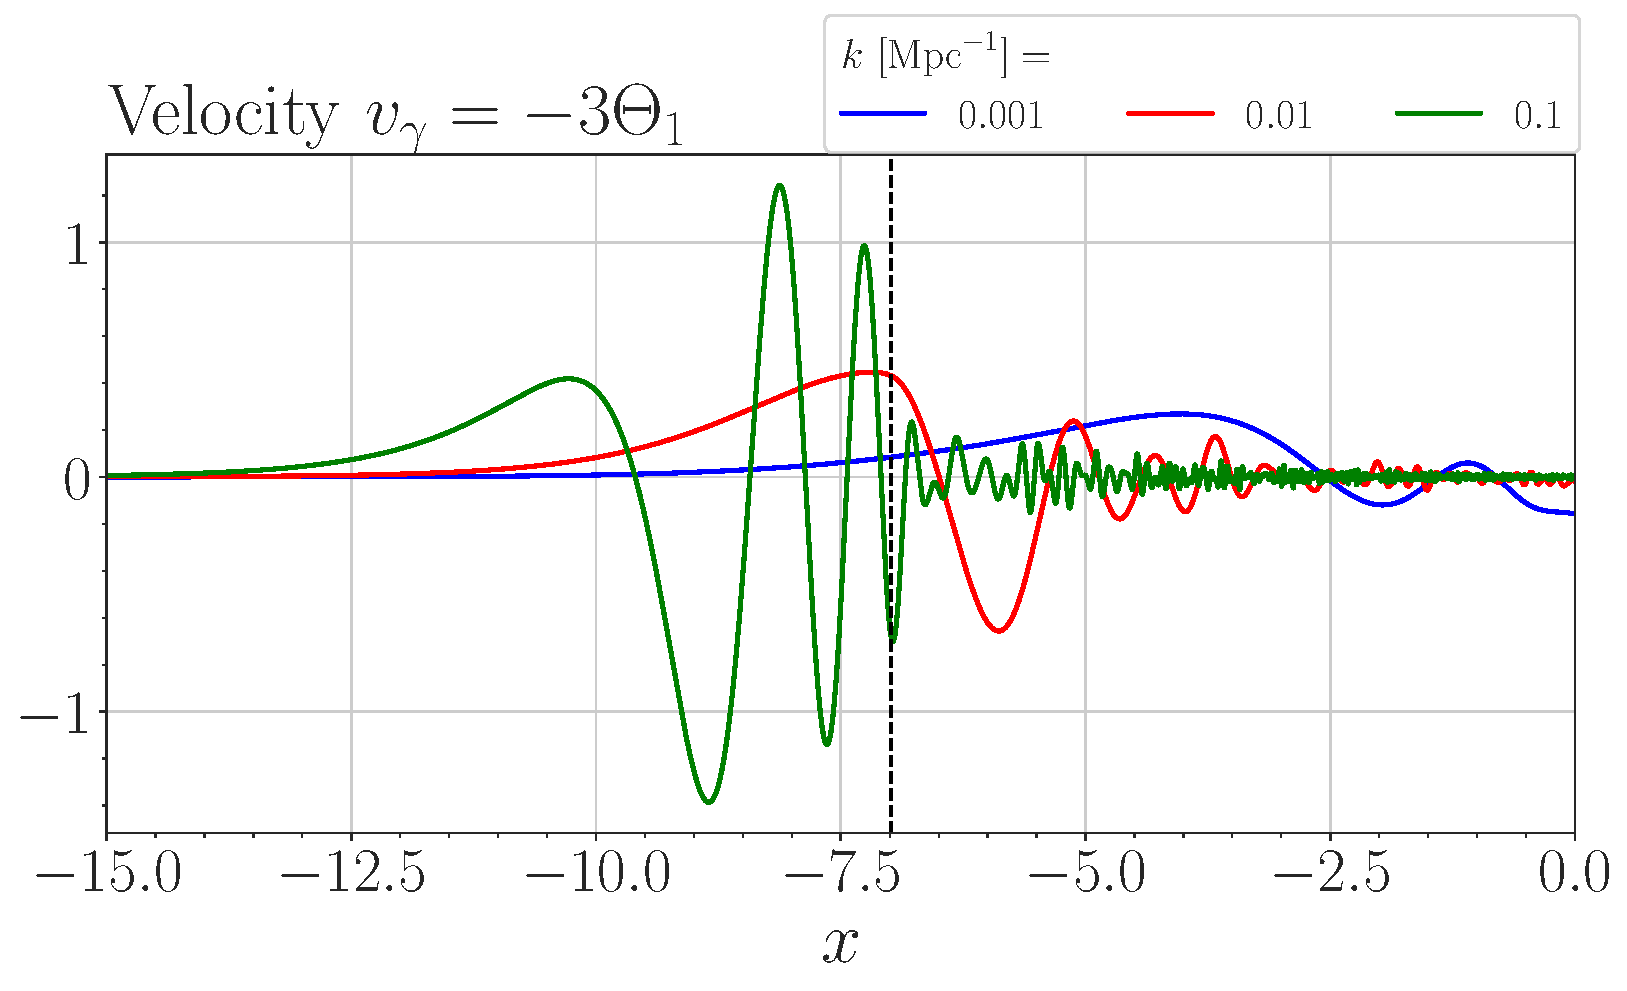
\includegraphics[width=\linewidth]{dipole.pdf}
        \caption{Photon velocity represented by the photon dipole for the various $k$-mdoes. Recombination is marked as a shaded grey area. The time of radiation-matter equality is marked with a dashed black line.}
        \label{fig:m3:dipole}
    \end{figure}

    The same is the case for the quadrupole in ~\cref{fig:m3:quadrapole}. However, as previously assumed, the quadrupole term is strongly suppressed during tight coupling, but behave similarly to the lower order multipoles after tight coupling. This is because during tight coupling, the photon-baryon plasma behaved very much like a fluid, only described by some average temperature and a velocity. Hence, there were no significant quadrupole (or any higher order multipole) moment(s) in this regime. Considering the large and intermediate scale modes (blue and red curve) we are able to close the discussion of the sum of potential in ~\cref{fig:m3:potentials}, where the quadrupole was the main contributor to the sinusoidal frequency, and $k$ to the amplitude. The small scales modes of the quadrupole experience the same diffusion damping as the lower multipoles. 

    \begin{figure}
        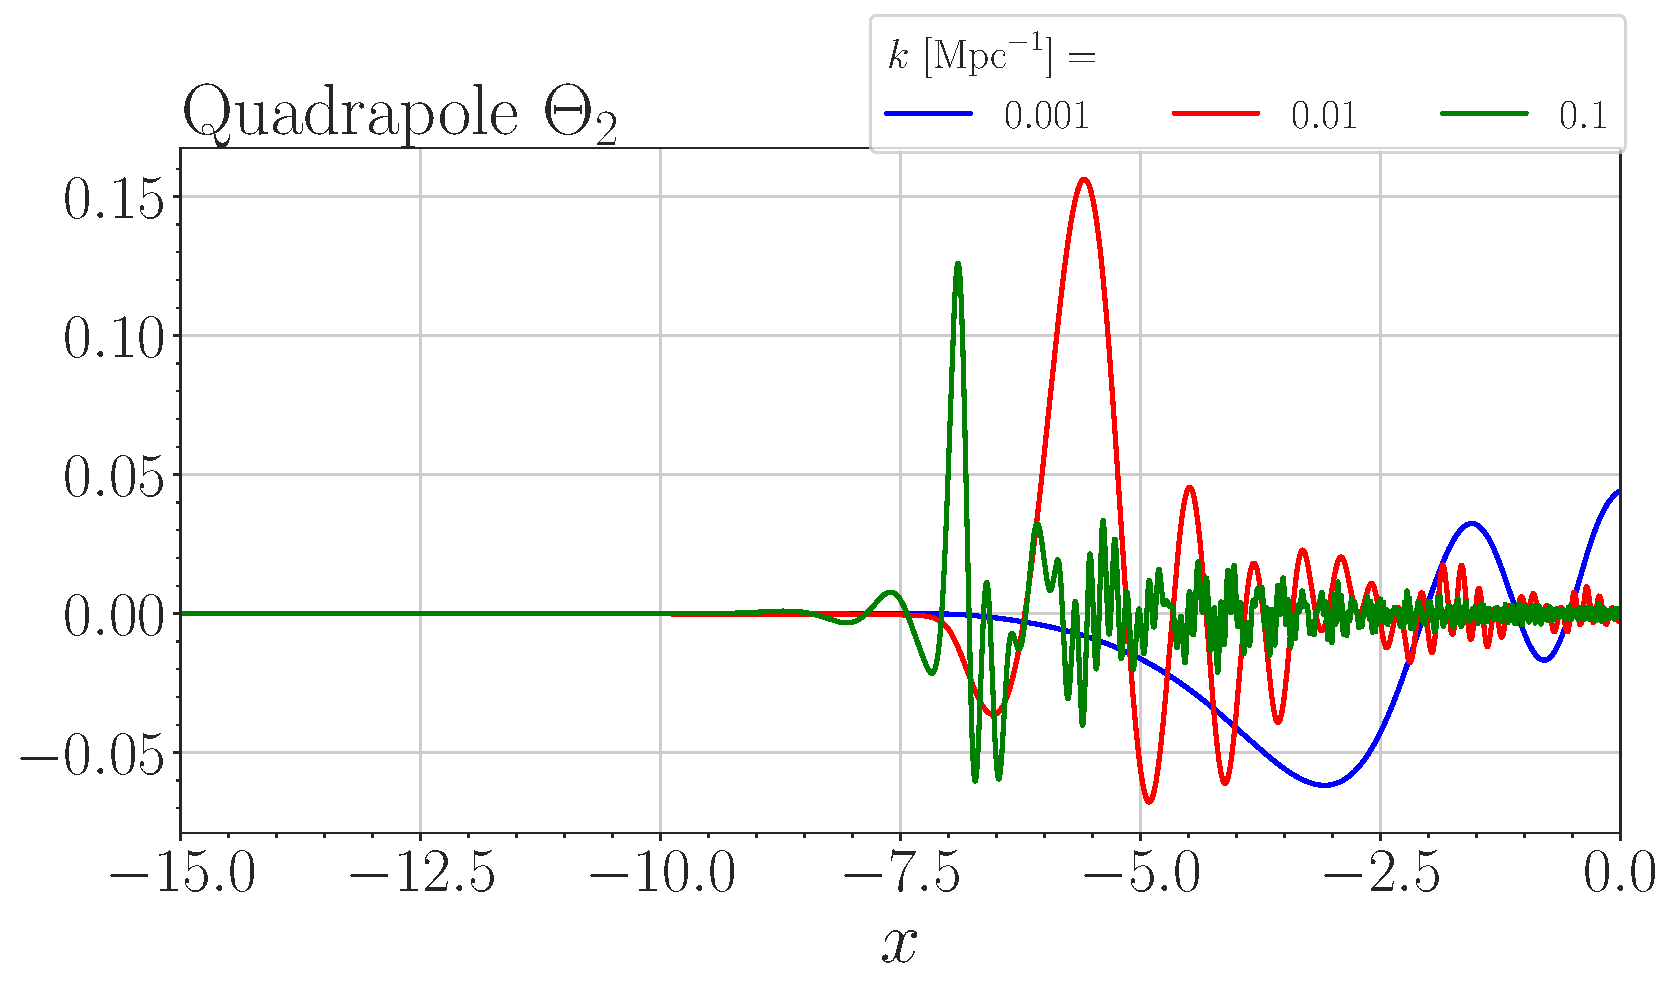
\includegraphics[width=\linewidth]{quadrapole.pdf}
        \caption{Quadrapole term of the photon perturbation. This term only becomes relevant after tight coupling. Recombination is marked as a shaded grey area. The time of radiation-matter equality is marked with a dashed black line.}
        \label{fig:m3:quadrapole}
    \end{figure}

\subsubsection{Matter perturbations}

    ~\cref{fig:m3:delta} show the overdensities of cold dark matter and baryons as function of time $x$, for the various $k$-modes. The small scale mode (green) enter the horizon during radiation domination, and immediately begins to cluster in overdense regions. The cold dark matter is not coupled to anything so its overdensity evolves on its own, only restricted by the growth of the Universe itself. During radiation domination, the rapid expansion of the universe makes the evolution of the cold dark matter logarithmic. Baryons, on the other hand, are coupled to photons and experiences photon radiation pressure which prevent their overdensities from growing. Instead, the interplay between radiation pressure and gravitation propagates acoustic sound waves in the plasma, manifest as oscillations in Fourier space. These are seen in the plot (green dashed line). These oscillations will continue as long as photons and baryons are coupled. As we transition from radiation to matter dominated, the evolution of the dark matter overdensity change from a logarithmic relationship to a power law scaling with the scale factor $a$. This is because the expansion rate of the Universe change alongside its dominant constituent, and when matter becomes dominant, the expansion rate decreases. This enables larger perturbations in the dark matter. The behaviour of the baryons change once they decouple from the photons. Now they do not feel the same radiation pressure as before, so they start to gather in the potential already in existence due to dark matter. This happens slightly after decoupling. There is a small delay due to compton drag, photons diffuse and scatter of baryons, and the baryons already have some velocity from the oscillation. \footnote{The width of the grey shaded area showing recombination cannot be taken literally as it is there just to showcase the fact that recombination and decoupling are not instantaneous processes.} From now on, the baryons fall into the gravitational wells, and all matter evolve together deep in matter domination. Close to $x=0$, when dark energy become the dominant constituent, the acceleration of the universe increases and the matter overdensities grow slower because of this.

    The intermediate scale mode enters the horizon around the time of radiation matter equality, so the baryons deviate slightly from the dark matter evolution. However, there is not any oscillatory behaviour since this mode did not enter the horizon early enough to capture the oscillations of the plasma. During matter dominating, all matter evolves similarly; growing as a power law w.r.t. the scale factor. The blue line representing large scale modes show this, entering the horizon deep in matter domination and immediately starts to grow according to this power law. 
    


    % For the matter perturbations, we start with the overdensities for cold dark matter and baryons, shown in ~\cref{fig:m3:delta}. Intuitively, we would expect small fluctuations in density to occur at very small scales early on, and then at larger scales gradually as the horizon increase. During the radiation dominated regime, expect the matter densities to be relatively homogenous on large scales, but noticeable on small scaler. In the matter dominated regime we expect overdense regions to attract more and more matter, increasing the overdensities. These effect should be noticeable on larger scales even, i.e. the modes that undergo horizon crossing during matter dominatin. When inspecting ~\cref{fig:m3:delta} this is indeed what we observe. The overdensity of the small scale mode in green starts to increase during radiation domination, large scale mode in blue during matter domination and the intermediate scale mode in red somewhere in between. All modes increase during matter domination which is what we expected. During dark energy domination we would expect the acceleration of the Universe to start to break up some structures and decrease the horizon, which would also decrease the matter overdensities. Lastly, we take note of the oscillations in the baryon density right before and after matter-radiation equality, but save the discussion for later. 

    \begin{figure}
        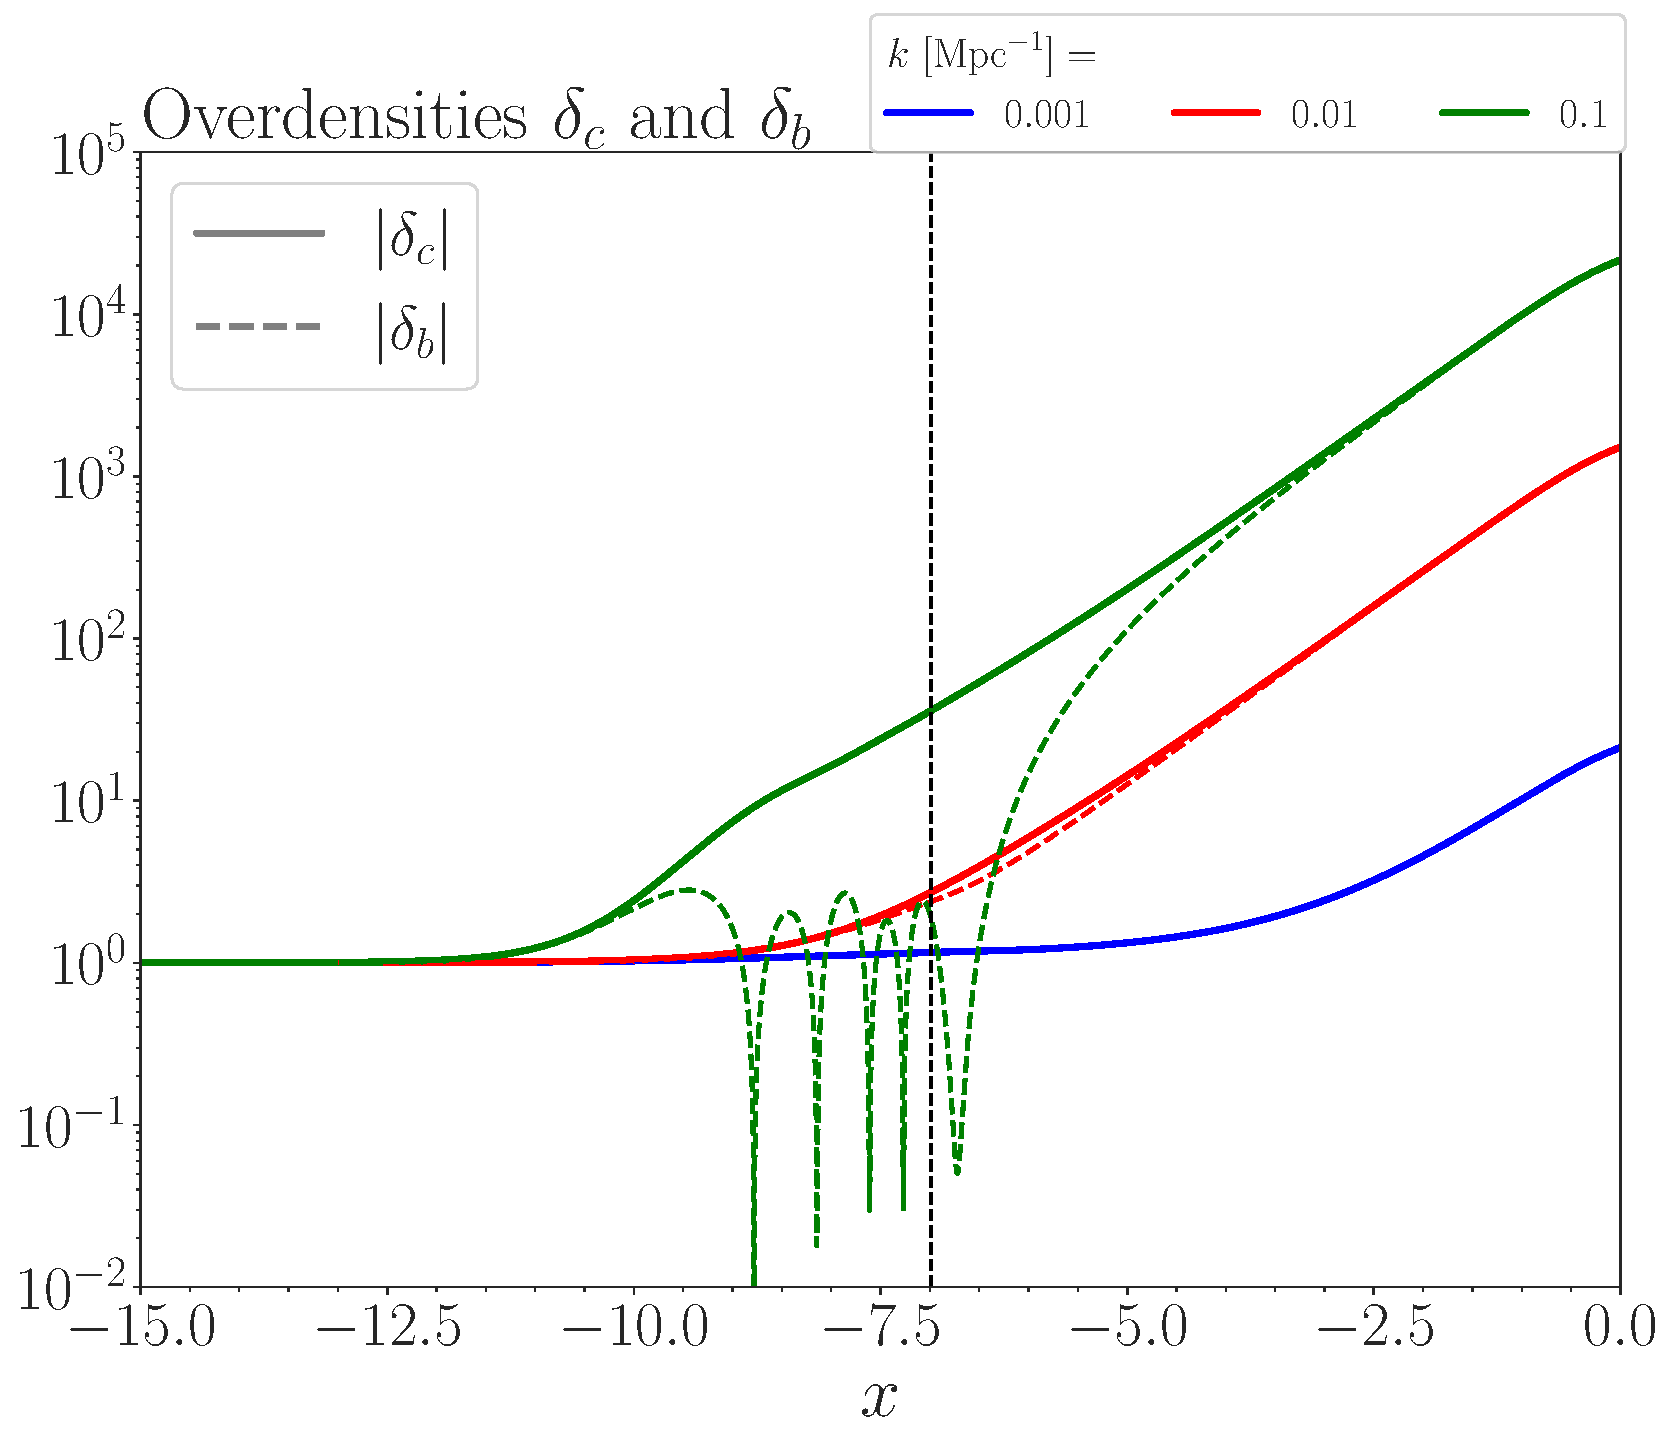
\includegraphics[width=\linewidth]{delta.pdf}
        \caption{The overdensities of cold dark matter and baryons for the various $k$-modes. Recombination is marked as a shaded grey area. The time of radiation-matter equality is marked with a dashed black line.}
        \label{fig:m3:delta}
    \end{figure}
    
    We emphasise the above discussion by considering only the small scale mode, and including the photon overdensity as well. This is shown in ~\cref{fig:m3:delta_comparison}. We recognise the dark matter and baryon overdensities, and we also clearly see the coupling between baryons and photons at early times, before recombination. After this, the baryon evolves as the dark matter, and the photons diffuse, reducing the amplitude of their oscillations, effectively smoothing their overdensitites. This diffusion drags out the time it takes for the baryons to fall in to the potentials (to keep up with dark matter). This is the effect of Compton drag, as diffusion is effectively photons interacting with electrons through Compton scattering, with an increased mean free path between each interaction. 

    \begin{figure}
        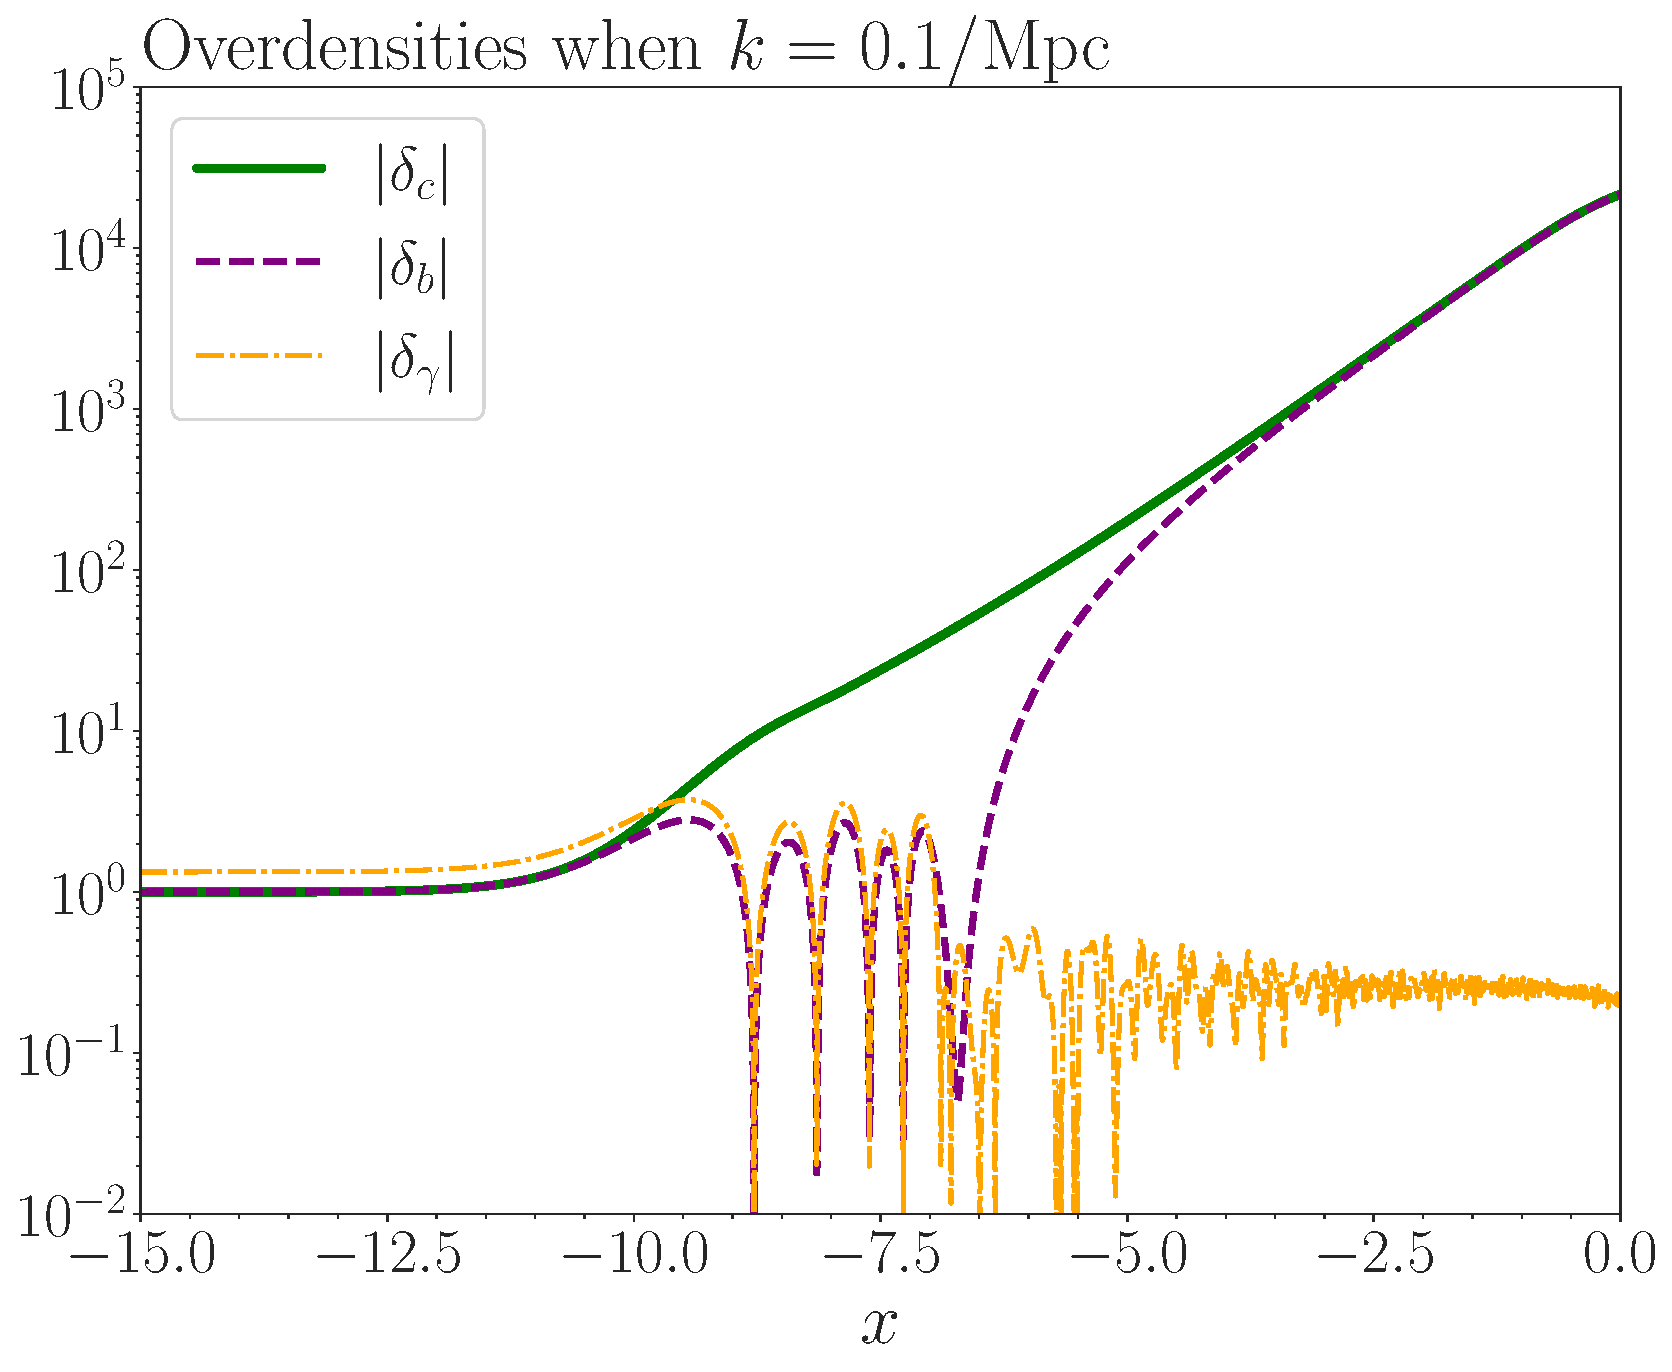
\includegraphics[width=\linewidth]{delta_comparison.pdf}
        \caption{Comparison of the overdensities of cold dark matter, baryons and photons for a small scale mode. We clearly see the decoupling of photons from baryons during recombination, which is marked as a shaded grey area. The time of radiation-matter equality is marked with a dashed black line. }
        \label{fig:m3:delta_comparison}
    \end{figure}
    
    
    % The remaining question to answer now is why does the baryon overdensity and velocity oscillate for the modes entering the horizon during radiation domination? In order to answer this question we consider the largest mode among the three; $k=0.1$/Mpc, and plot the velocities and overdensities of the cold dark matter, baryons and photons in the same plot. The result is seen in ~\cref{fig:m3:velocity_comparison} for the velocities and in ~\cref{fig:m3:delta_comparison} for the overdensities. We have already made statements about the oscillation of the photon velocity from ~\cref{fig:m3:dipole}, and photon overdensity from ~\cref{fig:m3:monopole}. The most important time in ~\cref{fig:m3:velocity_comparison} and ~\cref{fig:m3:delta_comparison} is the time of recombination (dashed line), which is closely related to the time of decoupling and last scattering, when the photons decouple from the baryons. Before this, baryons and photons are tightly coupled so we expect them to evolve similarly. It therefore makes sense that we have oscillations in the baryon velocity and overdensity before recombinations, as the baryons were tightly coupled to the photons. After decoupling, the baryon velocity and overdensity show similar behaviour to those of cold dark matter. At the same time, the oscillations of the photon monopole and dipole causes the photon velocity and overdensity to gradually decrease and converge as the photons free stream through the Universe. 

    ~\cref{fig:m3:velocity} show the velocities (bulk velocity of the fluid motion) of the cold dark matter and baryons. We start by noticing that for super-horizon scales (to the left of the plot), the velocities are the same for baryons and cold dark matter, and it follows the expansion of the Universe. It must be so, because no physics can affect the velocity which must be comoving as the Universe expands. For scales entering the horizon at late times it is always like this (blue line); the velocity follows the expansion of the Universe since the physical overdensity is in the same comoving location (for large scales). For baryons entering the horizon during radiation domination (small scales) it is a different story as this is an acoustic wave travelling outwards with some velocity. This is captured as oscillations in ~\cref{fig:m3:velocity}. The cold dark matter overdensities for small scales will also have a bulk velocity relative to the comoving coordinate system as these overdensities are subjected to the changing potentials. ~\cref{fig:m3:velocity_comparison} compares the bulk velocities of cold dark matter, baryons and photons for a small scale mode. Once again we notice the decoupling of the photons after recombinations. This plots tells pretty much a similar story as ~\cref{fig:m3:delta_comparison}.

    \begin{figure}
        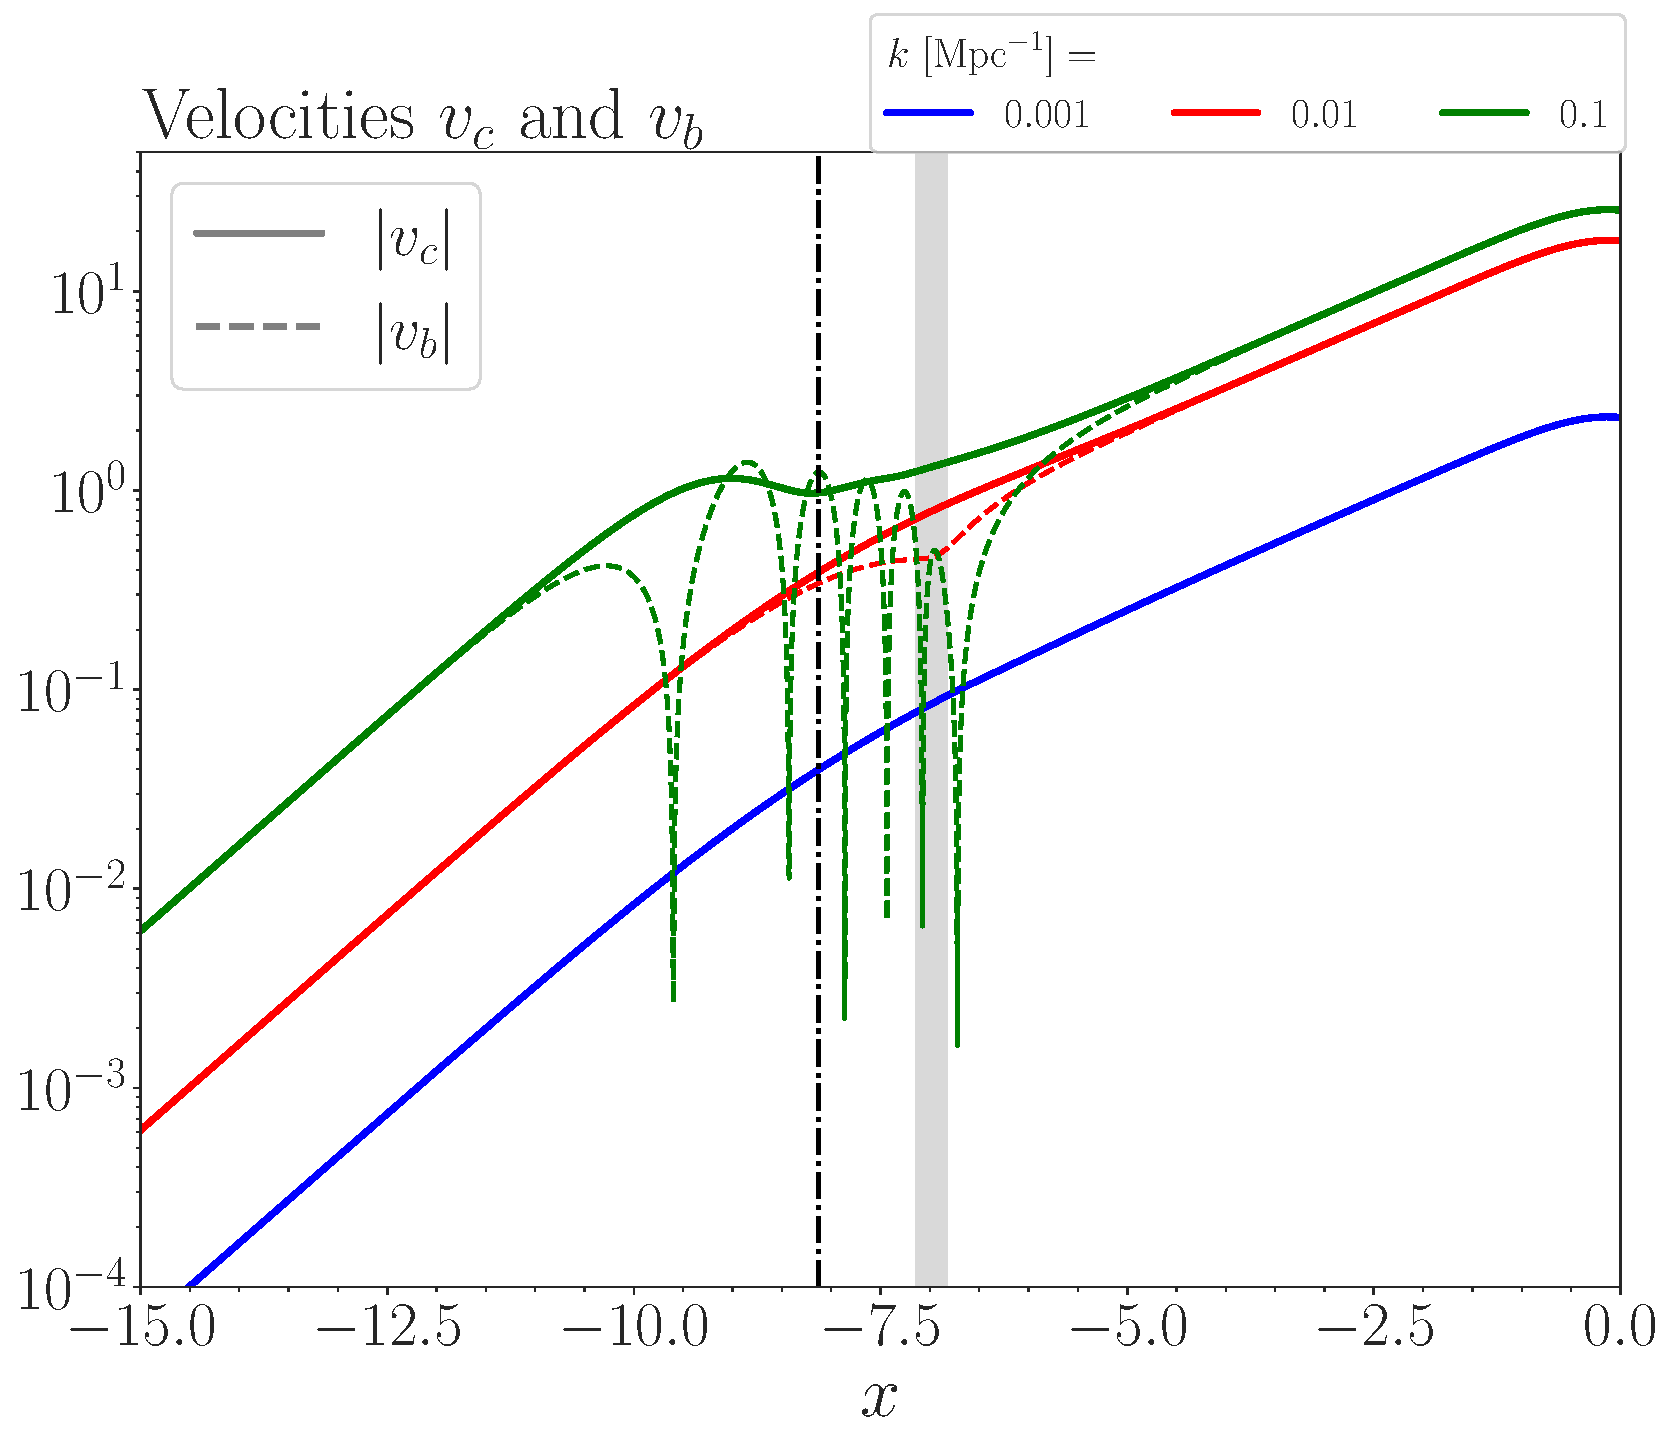
\includegraphics[width=\linewidth]{velocity.pdf}
        \caption{The bulk velocities of cold dark matter and baryons for the various $k$-modes. Recombination is marked as a shaded grey area. The time of radiation-matter equality is marked with a dashed black line.}
        \label{fig:m3:velocity}
    \end{figure}
    
    \begin{figure}
        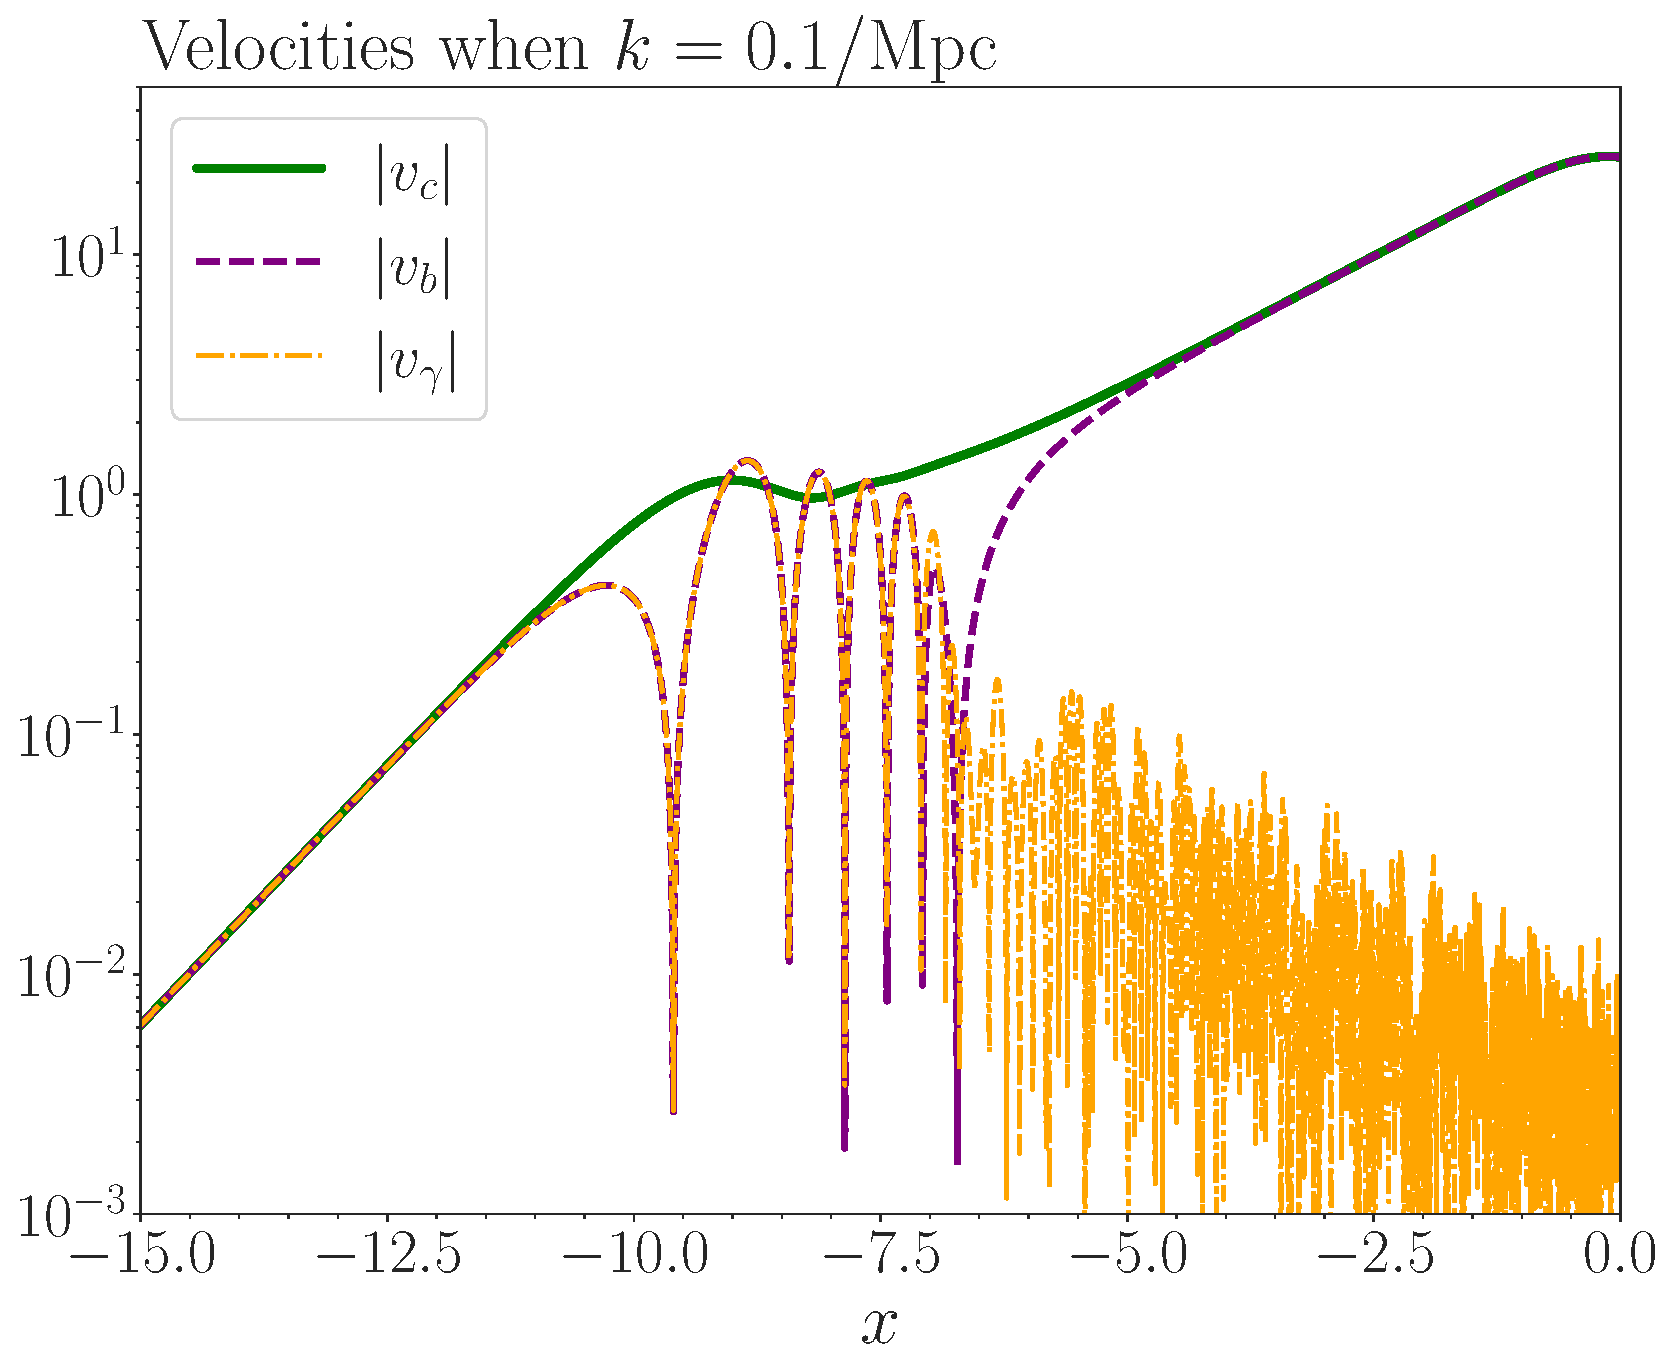
\includegraphics[width=\linewidth]{velocity_comparison.pdf}
        \caption{Comparison of the bulk velocities of cold dark matter, baryons and photons for a small scale mode. We clearly see the decoupling of photons from baryons during recombination, which is marked as a shaded grey area. The time of radiation-matter equality is marked with a dashed black line.}
        \label{fig:m3:velocity_comparison}
    \end{figure}
    

